%% Package and Class "uiucthesis2014" for use with LaTeX2e.
\documentclass[edeposit,fullpage]{uiucthesis2018}


\usepackage[acronym,toc]{glossaries}
%\newacronym{<++>}{<++>}{<++>}
\newacronym[longplural={metric tons of heavy metal}]{MTHM}{MTHM}{metric ton of heavy metal}
\newacronym{ABM}{ABM}{agent-based modeling}
\newacronym{ACDIS}{ACDIS}{Program in Arms Control \& Domestic and International Security}
\newacronym{AEF}{AEF}{Averaged Eddington Factor}
\newacronym{AHTR}{AHTR}{Advanced High Temperature Reactor}
\newacronym{ANDRA}{ANDRA}{Agence Nationale pour la gestion des D\'echets RAdioactifs, the French National Agency for Radioactive Waste Management}
\newacronym{ANL}{ANL}{Argonne National Laboratory}
\newacronym{API}{API}{application programming interface}
\newacronym{ARDP}{ARDP}{Advanced Reactor Demonstration Program}
\newacronym{ARE}{ARE}{Aircraft Reactor Experiment}
\newacronym{ASME}{ASME}{American Society of Mechanical Engineers}
\newacronym{ATWS}{ATWS}{Anticipated Transient Without Scram}
\newacronym{BDBE}{BDBE}{Beyond Design Basis Event}
\newacronym{BIDS}{BIDS}{Berkeley Institute for Data Science}
\newacronym{BTE}{BTE}{Boltzmann transport equation}
\newacronym{BWR}{BWR}{boiling water reactor}
\newacronym{CAFCA}{CAFCA}{ Code for Advanced Fuel Cycles Assessment }
\newacronym{CAS}{CAS}{Chinese Academy of Sciences}
\newacronym{CDTN}{CDTN}{Centro de Desenvolvimento da Tecnologia Nuclear}
\newacronym{CEA}{CEA}{Commissariat \`a l'\'Energie Atomique et aux \'Energies Alternatives}
\newacronym{CFD}{CFD}{Computational Fluid Dynamics}
\newacronym{CI}{CI}{continuous integration}
\newacronym{CNEN}{CNEN}{Comiss\~{a}o Nacional de Energia Nuclear}
\newacronym{CNERG}{CNERG}{Computational Nuclear Engineering Research Group}
\newacronym{CNRS}{CNRS}{Centre National de la Recherche Scientifique}
\newacronym{COMSOL}{COMSOL}{COMmon SOLution}
\newacronym{COSI}{COSI}{Commelini-Sicard}
\newacronym{COTS}{COTS}{commercial, off-the-shelf}
\newacronym{CPM}{CPM}{collision probability method}
\newacronym{CSNF}{CSNF}{commercial spent nuclear fuel}
\newacronym{CTAH}{CTAHs}{Coiled Tube Air Heaters}
\newacronym{CUBIT}{CUBIT}{CUBIT Geometry and Mesh Generation Toolkit}
\newacronym{CURIE}{CURIE}{Centralized Used Fuel Resource for Information Exchange}
\newacronym{DAG}{DAG}{directed acyclic graph}
\newacronym{DANESS}{DANESS}{Dynamic Analysis of Nuclear Energy System Strategies}
\newacronym{DBE}{DBE}{Design Basis Event}
\newacronym{DES}{DES}{Detached eddy simulation}
\newacronym{DESAE}{DESAE}{Dynamic Analysis of Nuclear Energy Systems Strategies}
\newacronym{DF}{DF}{discontinuity factors}
\newacronym{DFEM}{DFEM}{discontinuous finite element method}
\newacronym{DG}{DG}{Discontinuous Galerkin}
\newacronym{DHS}{DHS}{Department of Homeland Security}
\newacronym{DNF}{DNF}{delayed neutron fraction}
\newacronym{DNP}{DNP}{delayed neutron precursor}
\newacronym{DNS}{DNS}{Direct numerical simulation}
\newacronym{DOE}{DOE}{Department of Energy}
\newacronym{DMSR}{DMSR}{Denatured Molten Salt Reactor}
\newacronym{DRACS}{DRACS}{Direct Reactor Auxiliary Cooling System}
\newacronym{DRE}{DRE}{dynamic resource exchange}
\newacronym{DSNF}{DSNF}{DOE spent nuclear fuel}
\newacronym{DYMOND}{DYMOND}{Dynamic Model of Nuclear Development }
\newacronym{EBS}{EBS}{Engineered Barrier System}
\newacronym{EDZ}{EDZ}{Excavation Disturbed Zone}
\newacronym{EPA}{EPA}{Environmental Protection Agency}
\newacronym{EP}{EP}{Engineering Physics}
\newacronym{EVOL}{EVOL}{Evaluation and Viability of Liquid Fuel Fast Reactor System}
\newacronym{FCO}{FCO}{Fuel Cycle Options}
\newacronym{FCT}{FCT}{Fuel Cycle Technology}
\newacronym{FEHM}{FEHM}{Finite Element Heat and Mass Transfer}
\newacronym{FEM}{FEM}{finite element method}
\newacronym{FEPs}{FEPs}{Features, Events, and Processes}
\newacronym{FHR}{FHR}{Fluoride-Salt-Cooled High-Temperature Reactor}
\newacronym{FLiBe}{FLiBe}{Fluoride-Lithium-Beryllium}
\newacronym{FP}{FP}{fission product}
\newacronym{FVM}{FVM}{finite volume method}
\newacronym{GDSE}{GDSE}{Generic Disposal System Environment}
\newacronym{GDSM}{GDSM}{Generic Disposal System Model}
\newacronym{GENIUSv1}{GENIUSv1}{Global Evaluation of Nuclear Infrastructure Utilization Scenarios, Version 1}
\newacronym{GENIUSv2}{GENIUSv2}{Global Evaluation of Nuclear Infrastructure Utilization Scenarios, Version 2}
\newacronym{GENIUS}{GENIUS}{Global Evaluation of Nuclear Infrastructure Utilization Scenarios}
\newacronym{GET}{GET}{general equivalence theory}
\newacronym{GIF}{GIF}{Generation IV International Forum}
\newacronym{GPAM}{GPAM}{Generic Performance Assessment Model}
\newacronym{GRSAC}{GRSAC}{Graphite Reactor Severe Accident Code}
\newacronym{GUI}{GUI}{graphical user interface}
\newacronym{HALEU}{HALEU}{high-assay low-enriched uranium}
\newacronym{HLW}{HLW}{high level waste}
\newacronym{HPC}{HPC}{high-performance computing}
\newacronym{HTC}{HTC}{high-throughput computing}
\newacronym{HTGR}{HTGR}{High-Temperature Gas-Cooled Reactor}
\newacronym{IAEA}{IAEA}{International Atomic Energy Agency}
\newacronym{IDT}{IDT}{integrated diffusion/transport}
\newacronym{IEA}{IEA}{International Energy Agency}
\newacronym{IEMA}{IEMA}{Illinois Emergency Mangament Agency}
\newacronym{IHLRWM}{IHLRWM}{International High Level Radioactive Waste Management}
\newacronym{IMSBR}{IMSBR}{Indian Molten Salt Breeder Reactor}
\newacronym{IMSR}{IMSR}{Integral Molten Salt Reactor}
\newacronym{INL}{INL}{Idaho National Laboratory}
\newacronym{INS}{INS}{incompressible Navier-Stokes}
\newacronym{IO}{I/O}{input/output}
\newacronym{IPRR1}{IRP-R1}{Instituto de Pesquisas Radioativas Reator 1}
\newacronym{IRP}{IRP}{Integrated Research Project}
\newacronym{IRPhEP}{IRPhEP}{International Reactor Physics Benchmark Experiment Evaluation Project}
\newacronym{ISFSI}{ISFSI}{Independent Spent Fuel Storage Installation}
\newacronym{ISRG}{ISRG}{Independent Student Research Group}
\newacronym{JFNK}{JFNK}{Jacobian-Free Newton Krylov}
\newacronym{LANL}{LANL}{Los Alamos National Laboratory}
\newacronym{LBNL}{LBNL}{Lawrence Berkeley National Laboratory}
\newacronym{LCOE}{LCOE}{levelized cost of electricity}
\newacronym{LDRD}{LDRD}{laboratory directed research and development}
\newacronym{LES}{LES}{Large eddy simulation}
\newacronym{LEU}{LEU}{low-enriched uranium}
\newacronym{LFR}{LFR}{Lead-Cooled Fast Reactor}
\newacronym{LFMSR}{LFMSR}{Liquid-fueled Molten Salt Reactor}
\newacronym{LGPL}{LGPL}{GNU Lesser General Public License}
\newacronym{LLNL}{LLNL}{Lawrence Livermore National Laboratory}
\newacronym{LMFBR}{LMFBR}{Liquid Metal Fast Breeder Reactor}
\newacronym{LOFC}{LOFC}{Loss of Forced Cooling}
\newacronym{LOHS}{LOHS}{Loss of Heat Sink}
\newacronym{LOLA}{LOLA}{Loss of Large Area}
\newacronym{LP}{LP}{linear program}
\newacronym{LWR}{LWR}{Light Water Reactor}
\newacronym{MAGNOX}{MAGNOX}{Magnesium Alloy Graphie Moderated Gas Cooled Uranium Oxide Reactor}
\newacronym{MA}{MA}{minor actinide}
\newacronym{MCFR}{MCFR}{Molten Chloride Fast Reactor}
\newacronym{MCNP}{MCNP}{Monte Carlo N-Particle code}
\newacronym{MCRE}{MCRE}{Molten Chloride Reactor Experiment}
\newacronym{MECS}{MECS}{Method of Equivalent Cross Sections}
\newacronym{MILP}{MILP}{mixed-integer linear program}
\newacronym{MIT}{MIT}{the Massachusetts Institute of Technology}
\newacronym{MOAB}{MOAB}{Mesh-Oriented datABase}
\newacronym{MOOSE}{MOOSE}{Multiphysics Object-Oriented Simulation Environment}
\newacronym{MOSART}{MOSART}{Molten Salt Actinide Recycler and Transmuter}
\newacronym{MOX}{MOX}{mixed oxide}
\newacronym{MPI}{MPI}{Message Passing Interface}
\newacronym{MPM}{MPM}{Multi-Physics Modelling}
\newacronym{MRPP}{MRPP}{Multiregion Processing Plant}
\newacronym{MSBR}{MSBR}{Molten Salt Breeder Reactor}
\newacronym{MSFR}{MSFR}{Molten Salt Fast Reactor}
\newacronym{MSRE}{MSRE}{Molten Salt Reactor Experiment}
\newacronym{MSR}{MSR}{Molten Salt Reactor}
\newacronym{NAGRA}{NAGRA}{National Cooperative for the Disposal of Radioactive Waste}
\newacronym{NEAMS}{NEAMS}{Nuclear Energy Advanced Modeling and Simulation}
\newacronym{NEUP}{NEUP}{Nuclear Energy University Programs}
\newacronym{NFCSim}{NFCSim}{Nuclear Fuel Cycle Simulator}
\newacronym{NGNP}{NGNP}{Next Generation Nuclear Plant}
\newacronym{NMWPC}{NMWPC}{Nuclear MW Per Capita}
\newacronym{NNSA}{NNSA}{National Nuclear Security Administration}
\newacronym{NPP}{NPP}{Nuclear Power Plant}
\newacronym{NPRE}{NPRE}{Department of Nuclear, Plasma, and Radiological Engineering}
\newacronym{NQA1}{NQA-1}{Nuclear Quality Assurance - 1}
\newacronym{NRC}{NRC}{Nuclear Regulatory Commission}
\newacronym{NSF}{NSF}{National Science Foundation}
\newacronym{NSSC}{NSSC}{Nuclear Science and Security Consortium}
\newacronym{NUWASTE}{NUWASTE}{Nuclear Waste Assessment System for Technical Evaluation}
\newacronym{NWF}{NWF}{Nuclear Waste Fund}
\newacronym{NWTRB}{NWTRB}{Nuclear Waste Technical Review Board}
\newacronym{NZE}{NZE}{Net-Zero Emissions by 2050 Scenario}
\newacronym{OCRWM}{OCRWM}{Office of Civilian Radioactive Waste Management}
\newacronym{OOP}{OOP}{Object-oriented programming}
\newacronym{ORION}{ORION}{ORION}
\newacronym{ORNL}{ORNL}{Oak Ridge National Laboratory}
\newacronym{PARCS}{PARCS}{Purdue Advanced Reactor Core Simulator}
\newacronym{PBAHTR}{PB-AHTR}{Pebble Bed Advanced High Temperature Reactor}
\newacronym{PBFHR}{PB-FHR}{Pebble-Bed Fluoride-Salt-Cooled High-Temperature Reactor}
\newacronym{PDE}{PDE}{partial differential equation}
\newacronym{PEI}{PEI}{Peak Environmental Impact}
\newacronym{PH}{PRONGHORN}{PRONGHORN}
\newacronym{PoliMi}{PoliMi}{Politecnico di Milano}
\newacronym{PRIS}{PRIS}{Power Reactor Information System}
\newacronym{PRKE}{PRKE}{Point Reactor Kinetics Equations}
\newacronym{PSI}{PSI}{Paul Scherrer Institute}
\newacronym{PSPG}{PSPG}{Pressure-Stabilizing/Petrov-Galerkin}
\newacronym{PV}{PV}{photovoltaic}
\newacronym{PWAR}{PWAR}{Pratt and Whitney Aircraft Reactor}
\newacronym{PWR}{PWR}{Pressurized Water Reactor}
\newacronym{PyNE}{PyNE}{Python toolkit for Nuclear Engineering}
\newacronym{PyRK}{PyRK}{Python for Reactor Kinetics}
\newacronym{QA}{QA}{quality assurance}
\newacronym{QD}{QD}{quasi-diffusion}
\newacronym{RANS}{RANS}{Reynolds-averaged Navier-Stokes}
\newacronym{RDD}{RD\&D}{Research Development and Demonstration}
\newacronym{RD}{R\&D}{Research and Development}
\newacronym{REE}{REE}{rare earth element}
\newacronym{RELAP}{RELAP}{Reactor Excursion and Leak Analysis Program}
\newacronym{RIA}{RIA}{Reactivity Insertion Accident}
\newacronym{RIF}{RIF}{Region-Institution-Facility}
\newacronym{RMM}{RMM}{Response Matrix Method}
\newacronym{ROD}{ROD}{Reactor Optimum Design}
\newacronym{RSM}{RSM}{Reynolds stress model}
\newacronym{SAAF}{SAAF}{self-adjoint angular flux}
\newacronym{SAM}{SAM}{System Analysis Module}
\newacronym{SAMOFAR}{SAMOFAR}{Safety Assessment of the Molten Salt Fast Reactor}
\newacronym{SAMOSAFER}{SAMOSAFER}{Severe Accident Modeling and Safety Assessment for Fluid-fuel Energy Reactors}
\newacronym{SD}{SD}{standard deviation}
\newacronym{SFR}{SFR}{Sodium-Cooled Fast Reactor}
\newacronym{SINAP}{SINAP}{Shanghai Institute of Applied Physics}
\newacronym{SINDAG}{SINDA{\textbackslash}G}{Systems Improved Numerical Differencing Analyzer $\backslash$ Gaski}
\newacronym{SKB}{SKB}{Svensk K\"{a}rnbr\"{a}nslehantering AB}
\newacronym{SNF}{SNF}{spent nuclear fuel}
\newacronym{SNL}{SNL}{Sandia National Laboratory}
\newacronym{SPH}{SPH}{superhomogenization}
\newacronym{STC}{STC}{specific temperature change}
\newacronym{SUPG}{SUPG}{Streamline-Upwind/Petrov-Galerkin}
\newacronym{SVDC}{SVDC}{spatially varying diffusion coefficient}
\newacronym{SWF}{SWF}{Separations and Waste Forms}
\newacronym{SWU}{SWU}{Separative Work Unit}
\newacronym{TFM}{TFM}{Transient Fission Matrix}
\newacronym{TH}{TH}{thermal-hydraulics}
\newacronym{TMSR}{TMSR}{Thorium Molten Salt Reactor}
\newacronym{TRACE}{TRACE}{TRAC/RELAP Advanced Computational Engine}
\newacronym{TRIGA}{TRIGA}{Training Research Isotope General Atomic}
\newacronym{TRISO}{TRISO}{Tristructural Isotropic}
\newacronym{TRU}{TRU}{transuranic}
\newacronym{TSM}{TSM}{Total System Model}
\newacronym{TSPA}{TSPA}{Total System Performance Assessment for the Yucca Mountain License Application}
\newacronym{ThOX}{ThOX}{thorium oxide}
\newacronym{TUD}{TU Delft}{Technische Universiteit Delft}
\newacronym{UFD}{UFD}{Used Fuel Disposition}
\newacronym{UML}{UML}{Unified Modeling Language}
\newacronym{UOX}{UOX}{uranium oxide}
\newacronym{UQ}{UQ}{uncertainty quantification}
\newacronym{US}{US}{United States}
\newacronym{UW}{UW}{University of Wisconsin}
\newacronym{VISION}{VISION}{the Verifiable Fuel Cycle Simulation Model}
\newacronym{VSOP}{VSOP}{Very Superior Old Programs}
\newacronym{VVER}{VVER}{Voda-Vodyanoi Energetichesky Reaktor (Russian Pressurized Water Reactor)}
\newacronym{VV}{V\&V}{verification and validation}
\newacronym{WIPP}{WIPP}{Waste Isolation Pilot Plant}
\newacronym{YMR}{YMR}{Yucca Mountain Repository Site}
\newacronym{BOL}{BOL}{Beginning-of-Life}
\newacronym{ULOF}{ULOF}{Unprotected Loss of Flow}
\newacronym{LOSCA}{LOSCA}{Loss of Secondary Cooling Accident}
\newacronym{ULOHS}{ULOHS}{Unprotected Loss of Heat Sink}


\usepackage{xspace}
\usepackage{graphics}
\newcommand{\Cycamore}{\textsc{Cycamore}\xspace}
\newcommand{\Cyclus}{\textsc{Cyclus}\xspace}


\usepackage{placeins}
\usepackage{booktabs} % nice rules (thick lines) for tables
\usepackage{microtype} % improves typography for PDF

\usepackage[hyphens]{url}
\usepackage{hyperref}
\usepackage{subfig}
\usepackage{hhline}
\usepackage{amsmath}
\usepackage{color}
\usepackage{multirow}
\usepackage{siunitx}
\sisetup{
    input-decimal-markers = .,input-ignore = {,},table-number-alignment = right,
    group-separator={,}, group-four-digits = true
}
\usepackage{fourier}
\usepackage{booktabs}
\newcommand\tab[1][1cm]{\hspace*{#1}}

\usepackage{threeparttable, tablefootnote}

%tikzpicture fit to page width
\usepackage{environ}
\makeatletter
\newsavebox{\measure@tikzpicture}
\NewEnviron{scaletikzpicturetowidth}[1]{%
  \def\tikz@width{#1}%
  \def\tikzscale{1}\begin{lrbox}{\measure@tikzpicture}%
  \BODY
  \end{lrbox}
  \pgfmathparse{#1/\wd\measure@tikzpicture}%
  \edef\tikzscale{\pgfmathresult}%
  \BODY
}

\usepackage{tabularx}
\newcolumntype{b}{>{\hsize=1.0\hsize}X}
\newcolumntype{q}{>{\hsize=0.5\hsize}X}
\newcolumntype{R}{>{\raggedleft\arraybackslash\hsize=0.5\hsize}X}
\newcolumntype{z}{>{\hsize=0.75\hsize}X}
\newcolumntype{s}{>{\hsize=.5\hsize}X}
\newcolumntype{m}{>{\hsize=.75\hsize}X}

\usepackage{cleveref}
\usepackage{datatool}
\usepackage[numbers]{natbib}
\usepackage{notoccite}


\usepackage{tikz}
\usetikzlibrary{positioning, arrows, decorations, shapes}

\usetikzlibrary{shapes.geometric,arrows}
\tikzstyle{process} = [rectangle, rounded corners, minimum width=2.5cm, minimum height=1cm,text centered, draw=black, fill=blue!30]

\tikzstyle{object} = [ellipse, rounded corners, minimum width=3cm, minimum height=1cm,text centered, draw=black, fill=green!30]
\tikzstyle{objectr} = [ellipse, rounded corners, minimum width=3cm, minimum height=1cm,text centered, draw=black, fill=red!30]

\tikzstyle{empty} =  [rectangle, rounded corners, minimum width=2.5cm, minimum height=0.7cm,text centered, draw=black, fill=white!30]
\tikzstyle{arrow} = [thick,->,>=stealth]


\title{Example Template}
\author{Charles Bae}
\department{Nuclear, Plasma, Radiological Engineering}
\schools{B.S., University of Illinois - Urbana Champaign, 2017}
\msthesis
\advisor{Kathryn D. Huff}
\degreeyear{2018}
\committee{Assistant Professor Kathryn D. Huff, Adviser \\ Professor Segundo Lector }


\begin{document}
\maketitle

\frontmatter
%% Create an abstract that can also be used for the ProQuest abstract.
%% Note that ProQuest truncates their abstracts at 350 words.
\begin{abstract}

Abstract.

\end{abstract}

\chapter*{Acknowledgments}

Acks.

%% The thesis format requires the Table of Contents to come
%% before any other major sections, all of these sections after
%% the Table of Contents must be listed therein (i.e., use \chapter,
%% not \chapter*).  Common sections to have between the Table of
%% Contents and the main text are:
%%
%% List of Tables
%% List of Figures
%% List Symbols and/or Abbreviations
%% etc.

\tableofcontents
\listoftables
\listoffigures

%% Create a List of Abbreviations. The left column
%% is 1 inch wide and left-justified
%\chapter{List of Abbreviations}
%\printglossaries
%% Create a List of Symbols. The left column
%% is 0.7 inch wide and centered

\pagebreak
\mainmatter

\chapter{Introduction}
\section{Motivation}

A liquid-fueled \gls{MSR} is an advanced nuclear reactor with fissile material
dissolved in a molten salt mixture. This fuel salt mixture doubles as the primary reactor coolant
for transferring heat from the reactor core to the primary heat exchangers. Figure \ref{fig:msr}
shows a schematic diagram of a thermal-spectrum, channel-type \gls{MSR}. In channel-type
\glspl{MSR}, the fuel salt flows through vertical channels in the reactor core alongside neutron
moderators (e.g., graphite, heavy water, or molten sodium hydroxide). 
%
\begin{figure}[htb!]
	\centering
	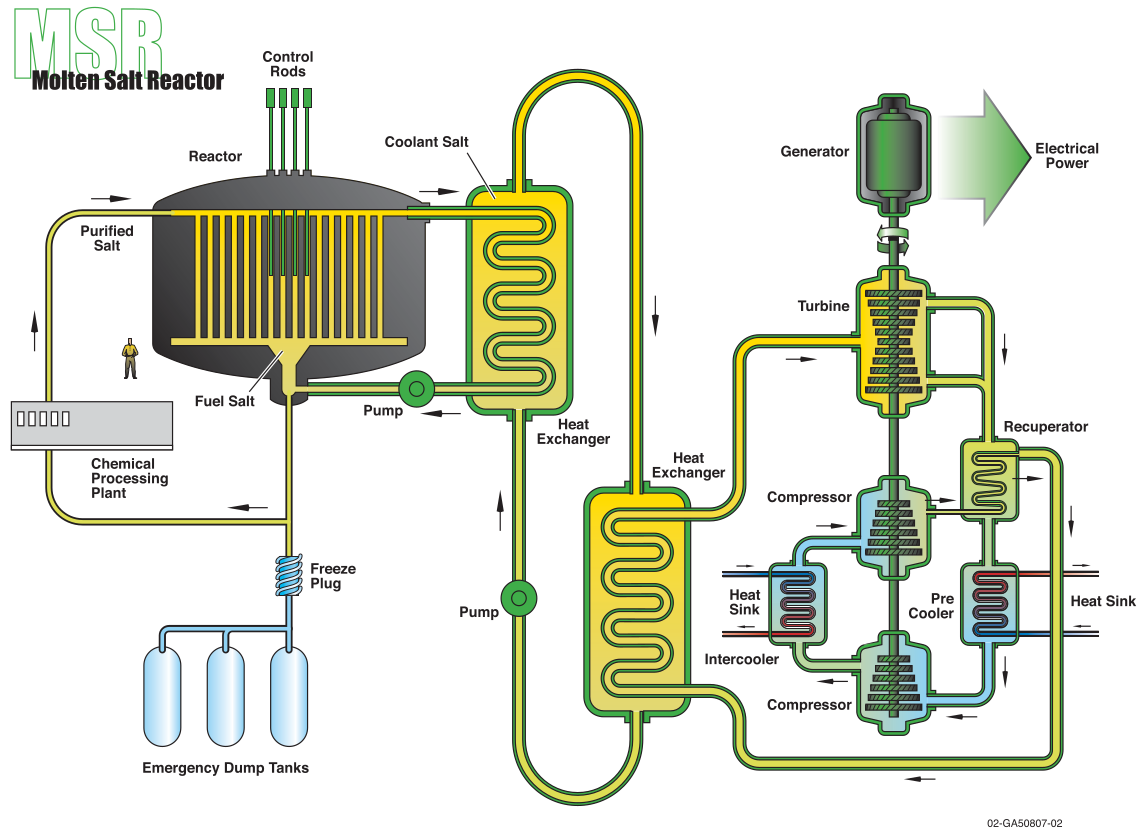
\includegraphics[width=.7\columnwidth]{msr}
	\caption{Schematic diagram of the \gls{MSR} concept. Retrieved from
	\cite{u.s._doe_nuclear_energy_research_advisory_committee_technology_2002}.}
	\label{fig:msr}
\end{figure}

The \gls{MSR} is one of six advanced reactor concepts selected for improved safety, sustainability,
efficiency, and cost over the current generation of predominantly \glspl{LWR} at the \gls{GIF}
\cite{u.s._doe_nuclear_energy_research_advisory_committee_technology_2002}.
Due to the large fuel expansion coefficient, \glspl{MSR} possess an inherently robust
safety feature in the strong negative fuel temperature coefficient of
reactivity \cite{elsheikh_safety_2013}. This reactivity coefficient limits the
maximum temperature that the reactor core would experience in particular accident
scenarios, such as an unprotected reactivity insertion, because the subsequent
rise in core temperatures induces a significant drop in reactivity,
quickly neutralizing the initial reactivity insertion. \glspl{MSR} also
operate at a large thermal margin to boiling and can rely on natural
circulation in the event of a pump failure. For an additional layer of safety, many \gls{MSR}
designs incorporate a drain plug made of actively-cooled frozen salt, which
melts when the core temperatures exceed safety thresholds. Hot molten salt
in the core would then flow into a drain tank designed to hold the fuel salt in
a subcritical configuration to disrupt any further chain fission reactions.

Some \glspl{MSR}, like the \gls{MSBR} or the \gls{MSFR}, can
incorporate the thorium fuel cycle for improved sustainability arising from the
use of abundant natural thorium resources and reduced transuranic waste
\cite{heuer_towards_2014}. The latter consequence also reduces costs
associated with long-term nuclear waste storage. Online fuel reprocessing raises the capacity
factor by reducing reactor downtime during reactor operation \cite{dolan_1_2017}.
Molten salt coolant loops can operate at near atmospheric pressures which eliminates the need for a
thick pressure vessel and drives down construction costs. We can make further economic arguments
supporting \glspl{MSR} in the context of the
carbon-constrained future envisioned in the \gls{IEA}'s \gls{NZE} roadmap
\cite{iea_net_2021}. The roadmap for minimizing carbon emissions requires solar photovoltaic- and
wind-dominated energy markets, which can results in highly variable and non-dispatchable
electricity generation. The resulting volatility in electricity prices
encourages the construction of heat storage and peak power
production plants. At the same time, demand for carbon-neutral
fuel will rise as electrification is economically unfeasible
for some industries, such as the aviation and marine sectors, which depend on
energy-dense fuels for propulsion.
The most cost-efficient options for heat storage, peak power production, and carbon-neutral fuel
production all require high-temperature heat \cite{forsberg_market_2020}.
This requirement favors \glspl{MSR}, which can deliver heat at higher average
temperatures than \glspl{LWR} and \glspl{SFR}.

Significant hurdles still stand in the way of commercial \gls{MSR} deployment \cite{dolan_27_2017}.
Major technological challenges include the need for further research on \gls{MSR} safety analysis,
irradiation and corrosion behavior of \gls{MSR} structural components, fission product tracking
and processing, \gls{MSR} nuclear safeguards measures, and the development of \gls{MSR} hydraulic
and heat exchanger components.

\subsection{Past \& Present \gls{MSR} Research \& Development}

\gls{ORNL} researchers first conceived the \gls{MSR} concept in pursuit of a high-temperature
liquid fuel reactor for the US Aircraft Nuclear Propulsion program in
the 1950s \cite{rosenthal_molten-salt_1970}. They
built the first ever operational \gls{MSR}, the 2.5 MW$_{\text{th}}$
\gls{ARE} reactor at \gls{ORNL}. The successful demonstration of the \gls{ARE} spurred further
research into adapting \glspl{MSR} for civilian power generation \cite{rosenthal_molten-salt_1970}.
Continued \gls{MSR} research efforts culminated in designing constructing, and successfully
operating of the 8-MW$_{\text{th}}$, thermal-spectrum \gls{MSRE} with
graphite channels and a LiF-BeF$_2$-ZrF$_4$-UF$_4$ fuel salt mixture
\cite{haubenreich_experience_1970}. In addition to other operational achievements, the
\gls{MSRE} became the first reactor to run on $^{233}$U fuel bred from $^{232}$Th. Building on
their experience with the \gls{MSRE}, \gls{ORNL} proposed a new program for constructing and
operating a demonstration reactor based on the \gls{MSBR} concept
\cite{macpherson_molten_1985}. The \gls{MSBR} is a thermal-spectrum \gls{MSR} with fertile
$^{232}$Th isotopes mixed directly into the \gls{FLiBe} molten salt for $^{233}$U breeding. The
\gls{MSBR} was to rely on continuous online reprocessing to add fertile
material and remove fission product neutron poisons.
However, the \gls{MSBR} project was canceled prior to the demonstration stage in
favor of the \gls{LMFBR}, which had benefited from a longer development time and more substantial
political backing \cite{macpherson_molten_1985}.

Following a relative lull lasting until the late 1990s, renewed research efforts and interest from
the \gls{GIF}
provided new impetus for \gls{MSR} research and development. As of the end of 2024, numerous
\gls{MSR} designs exist at various stages of development. Leading \gls{MSR} designs, in terms of
development, licensing, or demonstration, include the \gls{MSFR} \cite{merle_optimized_2007},
\gls{MCFR} \cite{terrapower_terrapower_2021}, TMSR-LF1 \cite{zhang_review_2018}, and \gls{IMSR}
\cite{leblanc_18_2017}. The \gls{MSFR} is a fast-spectrum breeder reactor developed through
collaboration among European institutes with funding support from the
European Union. Figure \ref{fig:msfr} shows a schematic diagram of the \gls{MSFR}. As opposed to
the multi-channel design of the \gls{MSRE} and \gls{MSBR}, the \gls{MSFR} is a pool-type design and
the reactor core consists of a large molten salt pool without graphite moderators to avoid
frequent graphite replacements and positive graphite temperature reactivity feedback. The
\gls{MCFR} is a similar pool-type reactor under active development at TerraPower. TerraPower and
Southern Company embarked on a joint project to design, construct, and operate a prototype
\gls{MCRE} design with funding support from the \gls{DOE}'s \gls{ARDP}. \gls{CAS} launched the
\gls{TMSR} program in 2011 to develop and construct both solid-fueled and liquid-fueled \gls{TMSR}
designs \cite{zou_research_2019}. They finished construction of TMSR-LF1, a 2-MW$_{\text{th}}$
liquid-fueled prototype, in August 2021 and received approval for reactor commissioning in August
2022. Lastly, Canada-based Terrestrial Energy is also developing its \gls{IMSR}, a small modular
\gls{MSR} based on the \gls{MSRE}. It passed a joint technical review by
Canadian and US nuclear regulators in July 2022.

Developing \gls{MSR} simulation software plays a vital role in supporting \gls{MSR}
development. Accurate reactor modeling capabilities
accelerate reactor design and optimization by enabling quicker iteration through numerous design
changes. \gls{MSR} simulation software are also essential tools in reactor safety analysis and
licensing efforts since reactor developers must demonstrate and verify that the \gls{MSR} systems
perform as designed and remain safe under various accident scenarios. 
%
\begin{figure}[htb!]
	\centering
	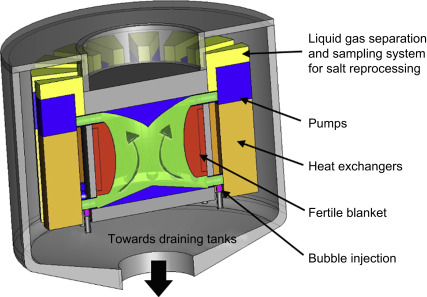
\includegraphics[width=.7\columnwidth]{msfr}
	\caption{Schematic diagram of the \gls{MSFR}. Retrieved from 
	\cite{allibert_7_2016}.}
	\label{fig:msfr}
\end{figure}

\subsection{Challenges in Multiphysics \gls{MSR} Modeling \& Simulation}

While modeling \glspl{MSR} is not necessarily more difficult than modeling
solid-fueled reactors, we must adapt our software tools to accurately model the
unique phenomena found in these circulating-fuel reactors. The differences in
the challenges of simulating \glspl{MSR} compared to solid-fueled reactors stem
primarily from the liquid fuel form of the fuel salt \cite{diamond_phenomena_2018,
huff_identifying_2019}.

Liquids generally exhibit greater thermal expansion per unit increase in temperature than solids.
The decreased fuel salt density due to thermal expansion
increases the likelihood of neutrons escaping the fuel region
and being absorbed by non-fissile material elsewhere in the reactor.
Consequently, combined with the temperature-dependent Doppler broadening of
resonance capture cross sections, \glspl{MSR} possess stronger negative fuel
temperature reactivity feedback than their solid-fueled counterparts
\cite{elsheikh_safety_2013}. These
phenomena ultimately result in strong interactions between the neutron fluxes
and the fuel salt temperatures, given that neutron fluxes affect fuel salt temperatures
through fission heat generation and fuel salt temperatures affect neutron
fluxes through the mechanisms described previously.

With the fuel salt also providing cooling in the core through advective heat
transfer, velocity flow
profiles in the fuel salts strongly impact the temperature distribution via
advection-dominated heat transfer \cite{diamond_phenomena_2018}. The flow-driven
temperature distribution contrasts
with the relatively static temperature profiles in fuel pins and
other solid fuel types, which are physically separate from the coolant.

\Glspl{DNP} flow freely within the primary coolant loop instead of
being held in place as in solid-fueled reactors. Thus, the delayed neutron
source distribution varies significantly depending on the flow profile and
velocity of the salt. In addition, the reactor loses some delayed neutrons from out-of-core
\gls{DNP} decay. These delayed neutrons are considered lost as they are emitted
in subcritical regions and are unlikely to contribute to further fission
reactions in the active core. The reduced delayed neutron fraction in the core
contributes to a greater prompt power spike following a reactivity insertion
event than solid-fueled reactors, absent any temperature reactivity
feedback.

Molten-salt flow along various parts of the coolant loop may fall within the turbulent flow
regime, characterized by chaotic eddies, vortices, and other flow instabilities.
Turbulent flow effects further complicate multiphysics interactions of flow with the temperature
and \gls{DNP} distribution. Turbulent flow effects contribute significantly to advection-dominated
heat and particle transfer in molten salt systems, thereby causing enhanced mixing. Therefore,
multiphysics software for \gls{MSR} analysis require adequate flow modeling capabilities with
support for \gls{DNP} drift and some form of turbulence modeling.

\gls{MSR} simulation tools require transient modeling capabilities to simulate transient
accident scenarios. Furthermore, several transient scenarios involve control rods, either as active
safety mechanisms or as accident initiators through unintended control rod ejection. Therefore,
\gls{MSR} simulation tools also require accurate control rod modeling capabilities to run
numerical analyses of accident scenarios involving control rods.

\subsection{Moltres for Multiphysics \gls{MSR} Analysis}

Moltres \cite{lindsay_moltres_2017} is an open-source multiphysics reactor simulation software
explicitly developed considering \gls{MSR} characteristics in mind. Moltres is
built on the \gls{MOOSE} \cite{giudicelli_30_2024} open-source finite-element framework,
which facilitates multiphysics coupling between different
\gls{MOOSE}-based and \gls{MOOSE}-wrapped applications. The \gls{MOOSE} framework also provides
Moltres with advanced meshing and numerical solver capabilities through interfacing with libMesh
\cite{kirk_libmesh_2006} and PETSc \cite{satish_petsc_2019} open-source libraries. Therefore,
Moltres supports up to 3-D unstructured meshes, scales well on high-performance computing systems,
and provides a flexible multiphysics coupling system, which can be tailored for different types of
simulations.

Moltres models coupled neutronics and thermal-hydraulics in reactors. While
generally applicable to most reactor concepts, much of
Moltres' development focuses on meeting the needs of \gls{MSR} multiphysics simulations.
Together with \gls{MOOSE}'s \texttt{Heat}
\texttt{Conduction} and \texttt{Navier-Stokes} \cite{peterson_overview_2018}
modules, Moltres solves the multigroup neutron diffusion
equations for an arbitrary number of energy and precursor groups and
thermal-hydraulics equations simultaneously on the same mesh (or separately solved and coupled
through fixed-point iterations if desired).

Lindsay et al. \cite{lindsay_introduction_2018}
demonstrated Moltres' multiphysics \gls{MSR} modeling capabilities with 1-D salt
flow modeling in axisymmetric and 3-D models of the \gls{MSRE}. The neutron flux and
temperature distributions agreed qualitatively with legacy
\gls{MSRE} data albeit with some minor quantitative discrepancies due to
simplifications and assumptions in the reactor geometry. I demonstrated Moltres' capabilities for
1) looping of \gls{DNP} drift back into the reactor core, 2) coupling the \gls{DNP}
drift to numerically calculated salt flow profiles within the reactor core,
and 3) a decay heat model to simulate decay heat from fission products, with a 2-D axisymmetric
design of the \gls{MSFR} in my Master's thesis \cite{park_advancement_2020}.

While the Moltres
model of the \gls{MSFR} showed good agreement with other studies in most steady-state and transient
simulation cases, the Moltres model showed significant discrepancies during pump-initiated
transient scenarios without a proper turbulence model. Instead, the model applied a
uniform eddy viscosity assumption, which proved inadequate under non-steady flow. In order to
advance Moltres as a multiphysics simulation software for \gls{MSR} analysis, Moltres requires a
turbulence modeling capability to capture adequate turbulent flow phenomena and their interactions
with other physics present in \glspl{MSR}. Of the various classes of turbulence models, a
\gls{RANS}-based model is most suitable for coupling with Moltres when considering computational
efficiency. The \gls{RANS}-based equations are time-averaged fluid flow equations
derived by separating the flow variable into its time-averaged and fluctuating components.
\gls{RANS}-based models are also well-validated, representing the most widely used turbulence
models for engineering applications.

In addition to new features, Moltres would benefit from further \gls{VV} of its existing
multiphysics capabilities to identify software bugs and ensure reliable results. Accurate modeling
and simulation of salt flow-induced \gls{DNP} drift and the strong coupling between neutronics and
thermal-hydraulics are crucial for \gls{MSR} simulation tools.
% Therefore, the proposed work will include relevant \gls{VV} studies for Moltres.

\subsection{Control Rod Modeling in \glspl{MSR}}

While some \gls{MSR} concepts completely eliminated control rods from their signs, many still
retain them. Control rods consist of strong
neutron absorbers like boron, cadmium, or gadolinium to absorb and thus reduce the number of
neutrons available to contribute to further fission chain reactions. All reactors start operation
with excess reactivity to ensure enough fissile material is available to maintain power operation
and last through to the next scheduled refueling. Control rods and burnable poisons balance the
initial excess reactivity. Control rods are also helpful
for ramping the power up or down during start-up, shut-down, or load-following operations. Most
importantly, control rods provide a safety mechanism for quickly shutting down a reactor under
dangerous conditions. Rapid control rod insertion is the primary mechanism of a reactor scram to
reliably introduce a large negative reactivity insertion in response to an unintended reactivity
insertion or other events that may threaten the reactor's safe operation. 

Amongst other tasks in reactor modeling, reactor physics analysts aim to accurately reproduce
control rod worth, which is measured as the relative reduction
in the neutron multiplication factor $k_\text{eff}$ due to the insertion of the control rod in the
reactor. They are also interested in the accompanying change in flux shape near the
control rod. Neutrons entering the control rods are more likely to be absorbed than
adjacent regions in the reactor core. Therefore, control rods induce highly anisotropic neutron
angular fluxes and sharp gradients in the neutron flux in their vicinity. Control rods also cause
shifts in the neutron energy spectrum because their absorption cross sections are much higher in
the lower neutron energy range; more energetic neutrons generally have a higher probability of
escaping the control rod region. As a consequence, modeling control rods accurately requires
high-fidelity computational methods to capture the angular dependence in the neutron
flux near the highly absorbing medium. Existing reactor analysis workflows often rely on Monte
Carlo methods for high-fidelity neutron transport calculations.

However, traditional neutron transport methods, including Monte Carlo methods, are computationally expensive
and thus are mainly used for time-independent neutronic analyses. For solid-fueled reactors,
static control rod analyses can be justified due to the relatively static temperature distribution
shape in the fuel and disparate timescales of heat transfer from the fuel to
the coolant (seconds) and neutron flux changes (microseconds to milliseconds). In
\glspl{MSR}, this distinction blurs due to molten salt serving the dual role of fuel and
coolant and the strong fuel temperature reactivity feedback. For time-dependent multiphysics
simulations coupling neutronics to \gls{TH} and other physics present in nuclear reactors, most
reactor analyses rely on neutron diffusion theory for modeling neutronics. The issue with applying
neutron diffusion theory near control rods arises because neutron diffusion theory approximates
neutron transport theory by integrating over the angular variables. As a result, diffusion-based
methods perform poorly in reactor systems with control rods.

% To tackle the issue of modeling control rods in \glspl{MSR} with the multigroup neutron diffusion
% solver in Moltres, I will develop and implement a novel hybrid method for incorporating neutron
% transport-derived corrections to the neutron diffusion method while largely preserving the
% computational efficiency of the neutron diffusion method over neutron transport methods. This will
% allow for computationally feasible transient analysis of \glspl{MSR} that incorporate thermal and
% neutronic feedback on variable timescales.

\section{Research Objectives and Outline}

The overarching goal of this work is to improve on Moltres as a reliable, intermediate-fidelity
simulation tool for multiphysics \gls{MSR} analysis that can be run on workstations as well as on
large leadership-class computing clusters. Thus, new and existing capabilities in Moltres must
be accurate within accepted bounds, rigorously verified, computationally efficient, and highly
scalable. These conditions form the underlying development principles of this work.

The scope of this dissertation can be divided into two main objectives.
%
%\begin{enumerate}[itemindent=20pt, listparindent=1.5em, label=\textbf{\arabic*}]
%  \item \textbf{Verification and validation of multiphysics capabilities in
%    Moltres}

    The first objective is to verify and validate multiphysics capabilities in Moltres for
    modeling and simulating
    the strong interactions between the neutronics and thermal-hydraulics in \glspl{MSR}. This
    will be accomplished through two separate studies: verifying Moltres against the CNRS
    benchmark \cite{tiberga_results_2020} for fast-spectrum \gls{MSR} analysis, and modeling the
    \gls{MSRE} zero-power pump start-up and coast-down experiments. I will perform the second study
    in collaboration with the developer of QuasiMolto \cite{reynolds_analysis_2023} as a \gls{VV}
    study.
%    with the additional aim of creating a reproducible numerical benchmark of the listed
%    \gls{MSRE} experiments.
%
%  \item \textbf{Implementation and verification of a \gls{RANS}-based turbulence model in Moltres}
    This objective includes implementing and verifying a Spalart-Allmaras turbulence model in
    Moltres to support future turbulent flow
    simulations for \gls{MSR} analyses. This will address the absence of turbulence modeling
    capability in Moltres and the consequent restriction on Moltres for modeling \gls{MSR} systems
    with complex turbulent flow.

%  \item \textbf{Development of a novel hybrid $S_N$-diffusion method for improved control rod modeling in Moltres}

    The second objective is to develop, implement, and demonstrate a novel hybrid $S_N$-diffusion
    method for accurate control rod modeling in
    time-dependent \gls{MSR} analyses. The hybrid method uses the discrete ordinates ($S_N$)
    neutron transport method to generate transport corrections in regions near control rods for
    drift correction terms in modified neutron diffusion equations. The $S_N$ method is applied on
    a reduced problem domain to ensure the hybrid method remains tractable on small to moderate
    computing clusters.
%\end{enumerate}

Chapter 2 presents a literature review of existing multiphysics \gls{MSR} simulation software,
\gls{VV} studies on \gls{MSR} modeling and simulation, turbulence modeling in \gls{MSR} systems,
and transport-correction techniques for neutron diffusion methods.
Chapter 3 provides an in-depth description of Moltres and its existing capabilities in the context
of previously published work. This chapter then presents Moltres \gls{VV} results for the CNRS
benchmark and the numerical \gls{MSRE} zero-power pump experiment studies. Following these studies,
the chapter presents the implementation and verification of the Spalart-Allmaras turbulence model
in Moltres.
Chapter 4 presents the theory and numerical implementation of the hybrid
$S_N$-diffusion method in Moltres. These include the $S_N$ method implementation, the transport
correction formulations, the iteration algorithm, the $S_N$-diffusion coupling implementation, and
general implementation details relating to the underlying numerical solver in Moltres.
Chapter 5 presents the verification and demonstration of the hybrid $S_N$-diffusion method for
$k_\text{eff}$ and rod worth calculations through
$k$-eigenvalue simulations of 1-D, 2-D, and 3-D \gls{MSRE} models. The hybrid method is verified
against reference results from OpenMC Monte Carlo neutron transport code and \gls{MSRE}
experimental data.
%Chapter 6 presents the demonstration of the hybrid $S_N$-diffusion method in time-dependent
%reactivity-initiated simulations modeling the \gls{MSRE} rod drop and reactivity insertion
%experiments.
Chapter 6 presents a demonstration of the hybrid $S_N$-diffusion method in a time-dependent
reactivity-initiated simulation modeling a \gls{MSRE} rod drop experiment.
Chapter 7 concludes this dissertation by summarizing the results presented, identifying limitations
in this work, and providing potential research directions to address those limitations or extend
this work.


\chapter*{Appendix}
%\appendix
\section{Additional data tables} \label{appendix:tables}

This Appendix presents observable values measured at nine
equidistant points along the centerlines AA' and BB' from Moltres and the
CNRS benchmark participants \cite{tiberga_results_2020}. We refer readers to
\cite{park_results_2021} and \cite{tiberga_results_2019} for the full set of
results from Moltres and the benchmark participants. 

\begin{table}[htbp!]
	\caption{Step 0.1 \textemdash\ Velocity components along centerlines AA' and BB'.}
	\centering
	\footnotesize
	\setlength\tabcolsep{1.5pt}
	\hspace*{-1cm}
	\renewcommand{\arraystretch}{.8}
	\begin{tabular}{c c c c c c c c c c c}
		\toprule
		\multirow{2}{*}{\textbf{Observable}} & \multirow{2}{*}{\textbf{Code}} & \multicolumn{9}{c}{\textbf{Results along $AA'$} (point coordinates are expressed in m)} \\
		& & {(0,1)} & {(0.25,1)} & {(0.5,1)} & {(0.75,1)} & {(1,1)} & {(1.25,1)} & {(1.5,1)} & {(1.75,1)} & {(2,1)} \\
		\midrule
		\multirow{5}{*}{$u_x$ (m s$^{-1}$)} & Moltres & 0.000E+00 & -1.923E-02 & -5.372E-02 & -8.371E-02 & -1.025E-01 & -1.043E-01 & -7.975E-02 & -3.080E-02 & 0.000E+00 \\
		& CNRS & 0.000E+00 & -1.924E-02 & -5.372E-02 & -8.369E-02 & -1.025E-01 & -1.043E-01 & -7.972E-02 & -3.080E-02 & 0.000E+00 \\
        & PoliMi & 0.000E+00 & -1.922E-02 & -5.365E-02 & -8.357E-02 & -1.023E-01 & -1.041E-01 & -7.947E-02 & -3.066E-02 & 0.000E+00 \\
        & PSI & 0.000E+00 & -1.929E-02 & -5.366E-02 & -8.332E-02 & -1.018E-01 & -1.034E-01 & -7.912E-02 & -3.072E-02 & 0.000E+00 \\
        & TUD & 1.002E-06 & -1.922E-02 & -5.372E-02 & -8.371E-02 & -1.025E-01 & -1.044E-01 & -7.977E-02 & -3.081E-02 & 4.198E-06 \\
        \midrule
		\multirow{5}{*}{$u_y$ (m s$^{-1}$)} & Moltres & 0.000E+00 & 7.269E-02 & 8.579E-02 & 6.087E-02 & 1.250E-02 & -4.794E-02 & -9.612E-02 & -8.722E-02 & 0.000E+00\\
		& CNRS & 0.000E+00 & 7.266E-02 & 8.575E-02 & 6.084E-02 & 1.251E-02 & -4.789E-02 & -9.606E-02 & -8.722E-02 & 0.000E+00 \\
        & PoliMi & 0.000E+00 & 7.139E-02 & 8.433E-02 & 6.007E-02 & 1.269E-02 & -4.691E-02 & -9.472E-02 & -8.621E-02 & 0.000E+00 \\
        & PSI & 0.000E+00 & 7.265E-02 & 8.534E-02 & 6.021E-02 & 1.230E-02 & -4.734E-02 & -9.536E-02 & -8.720E-02 & 0.000E+00 \\
        & TUD & 5.877E-06 & 7.269E-02 & 8.580E-02 & 6.089E-02 & 1.252E-02 & -4.794E-02 & -9.613E-02 & -8.726E-02 & -1.013E-05 \\
		\midrule
		\midrule
		\multirow{2}{*}{\textbf{Observable}} & \multirow{2}{*}{\textbf{Code}} & \multicolumn{9}{c}{\textbf{Results along $BB'$} (point coordinates are expressed in m)} \\
		& & {(1,0)} & {(1,0.25)} & {(1,0.5)} & {(1,0.75)} & {(1,1)} & {(1,1.25)} & {(1,1.5)} & {(1,1.75)} & {(1,2)} \\
		\midrule
		\multirow{5}{*}{$u_x$ (m s$^{-1}$)} & Moltres & 0.000E+00 & -3.518E-02 & -6.243E-02 & -8.723E-02 & -1.025E-01 & -8.770E-02 & -1.146E-02 & 1.718E-01 & 5.000E-01 \\
		& CNRS & 0.000E+00 & -3.517E-02 & -6.242E-02 & -8.720E-02 & -1.025E-01 & -8.766E-02 & -1.147E-02 & 1.717E-01 & 5.000E-01 \\
        & PoliMi & 0.000E+00 & -3.423E-02 & -6.107E-02 & -8.613E-02 & -1.023E-01 & -8.861E-02 & -1.299E-02 & 1.706E-01 & 5.000E-01 \\
        & PSI & 0.000E+00 & -3.511E-02 & -6.217E-02 & -8.667E-02 & -1.018E-01 & -8.731E-02 & -1.191E-02 & 1.705E-01 & 5.000E-01 \\
        & TUD & 1.494E-06 & -3.519E-02 & -6.244E-02 & -8.724E-02 & -1.025E-01 & -8.770E-02 & -1.146E-02 & 1.718E-01 & 5.000E-01 \\
        \midrule
		\multirow{5}{*}{$u_y$ (m s$^{-1}$)} & Moltres & 0.000E+00 & 5.161E-05 & 6.166E-04 & 3.842E-03 & 1.250E-02 & 2.525E-02 & 3.050E-02 & 1.501E-02 & 0.000E+00 \\
		& CNRS & 0.000E+00 & 5.641E-05 & 6.309E-04 & 3.862E-03 & 1.251E-02 & 2.524E-02 & 3.048E-02 & 1.500E-02 & 0.000E+00 \\
        & PoliMi & 0.000E+00 & 9.118E-05 & 7.484E-04 & 4.046E-03 & 1.269E-02 & 2.534E-02 & 3.050E-02 & 1.500E-02 & 0.000E+00 \\
        & PSI & 0.000E+00 & 7.727E-05 & 6.822E-04 & 3.875E-03 & 1.230E-02 & 2.472E-02 & 2.994E-02 & 1.481E-02 & 0.000E+00 \\
        & TUD & 1.501E-06 & 5.260E-05 & 6.209E-04 & 3.853E-03 & 1.252E-02 & 2.528E-02 & 3.053E-02 & 1.502E-02 & 7.987E-06 \\
		\bottomrule
	\end{tabular}
\end{table}

\begin{table}[htbp!]
	\caption{Step 0.2 \textemdash\ Fission rate density along $AA'$.}
	\centering
	\footnotesize
	\setlength\tabcolsep{1.5pt}
	\hspace*{-1cm}
	\renewcommand{\arraystretch}{.8}
	\begin{tabular}{c c c c c c c c c c c}
		\toprule
		\multirow{2}{*}{\textbf{Observable}} & \multirow{2}{*}{\textbf{Code}} & \multicolumn{9}{c}{\textbf{Results along $AA'$} (point coordinates are expressed in m)} \\
		& & {(0,1)} & {(0.25,1)} & {(0.5,1)} & {(0.75,1)} & {(1,1)} & {(1.25,1)} & {(1.5,1)} & {(1.75,1)} & {(2,1)} \\
		\midrule
		\multirow{7}{*}{\shortstack[1]{$\int_E \Sigma_f \Phi$d$E$\\(m$^{-3}$s$^{-1}$)}} & Moltres & 7.701E+17 & 7.461E+18
		& 1.303E+19 & 1.672E+19 & 1.801E+19 & 1.672E+19 & 1.303E+19 &
		7.461E+18 & 7.701E+17 \\
		& CNRS-$SP_1$ & 6.896E+17 & 7.436E+18 & 1.305E+19 & 1.678E+19 & 1.809E+19 & 1.678E+19 & 1.305E+19 & 7.436E+18 & 6.896E+17 \\
		& CNRS-$SP_3$ & 6.206E+17 & 7.450E+18 & 1.303E+19 & 1.673E+19 & 1.802E+19 & 1.673E+19 & 1.303E+19 & 7.450E+18 & 6.206E+17 \\
		& PoliMi & 7.780E+17 & 7.470E+18 & 1.310E+19 & 1.684E+19 & 1.815E+19 & 1.684E+19 & 1.310E+19 & 7.470E+18 & 7.780E+17 \\
		& PSI & 8.622E+17 & 7.436E+18 & 1.305E+19 & 1.678E+19 & 1.809E+19 & 1.678E+19 & 1.305E+19 & 7.436E+18 & 8.622E+17 \\
		& TUD-$S_2$ & 6.626E+17 & 7.433E+18 & 1.307E+19 & 1.682E+19 & 1.814E+19 & 1.682E+19 & 1.307E+19 & 7.433E+18 & 6.626E+17 \\
		& TUD-$S_6$ & 6.833E+17 & 7.463E+18 & 1.300E+19 & 1.667E+19 & 1.796E+19 & 1.667E+19 & 1.300E+19 & 7.463E+18 & 6.833E+17 \\
		\bottomrule
	\end{tabular}
\end{table}

\begin{table}[htbp!]
	\caption{Step 0.3 \textemdash\ Temperature distribution along centerlines $AA'$ and $BB'$.}
	\label{table:0.3}
	\centering
	\footnotesize
	\setlength\tabcolsep{1.5pt}
	\hspace*{-1cm}
	\renewcommand{\arraystretch}{.8}
	\begin{tabular}{c c c c c c c c c c c}
		\toprule
		\multirow{2}{*}{\textbf{Observable}} & \multirow{2}{*}{\textbf{Code}} & \multicolumn{9}{c}{\textbf{Results along $AA'$} (point coordinates are expressed in m)} \\
		& & {(0,1)} & {(0.25,1)} & {(0.5,1)} & {(0.75,1)} & {(1,1)} & {(1.25,1)} & {(1.5,1)} & {(1.75,1)} & {(2,1)} \\
		\midrule
		\multirow{7}{*}{$T$ (K)} & Moltres & 9.251E+02 & 1.194E+03 & 1.357E+03 & 1.361E+03 &
		1.303E+03 & 1.224E+03 & 1.131E+03 & 1.035E+03 & 9.251E+02 \\
		& CNRS-$SP_1$ & 9.253E+02 & 1.194E+03 & 1.358E+03 & 1.363E+03 & 1.305E+03 & 1.224E+03 & 1.131E+03 & 1.034E+03 & 9.251E+02 \\
		& CNRS-$SP_3$ & 9.236E+02 & 1.194E+03 & 1.357E+03 & 1.361E+03 & 1.304E+03 & 1.224E+03 & 1.131E+03 & 1.034E+03 & 9.235E+02 \\
		& PoliMi & 9.253E+02 & 1.196E+03 & 1.361E+03 & 1.364E+03 & 1.305E+03 & 1.224E+03 & 1.132E+03 & 1.035E+03 & 9.252E+02 \\
		& PSI & 9.253E+02 & 1.196E+03 & 1.356E+03 & 1.363E+03 & 1.306E+03 & 1.226E+03 & 1.133E+03 & 1.037E+03 & 9.252E+02 \\
		& TUD-$S_2$ & 9.212E+02 & 1.194E+03 & 1.359E+03 & 1.364E+03 & 1.305E+03 & 1.224E+03 & 1.131E+03 & 1.032E+03 & 9.225E+02 \\
		& TUD-$S_6$ & 9.219E+02 & 1.194E+03 & 1.356E+03 & 1.360E+03 & 1.303E+03 & 1.223E+03 & 1.131E+03 & 1.034E+03 & 9.233E+02 \\
		\midrule
		\midrule
		\multirow{2}{*}{\textbf{Observable}} & \multirow{2}{*}{\textbf{Code}} & \multicolumn{9}{c}{\textbf{Results along $BB'$} (point coordinates are expressed in m)} \\
		& & {(1,0)} & {(1,0.25)} & {(1,0.5)} & {(1,0.75)} & {(1,1)} & {(1,1.25)} & {(1,1.5)} & {(1,1.75)} & {(1,2)} \\
		\midrule
		\multirow{7}{*}{$T$ (K)} & Moltres & 9.251E+02 & 1.140E+03 & 1.272E+03 & 1.303E+03 &
		1.303E+03 & 1.313E+03 & 1.320E+03 & 1.264E+03 & 9.123E+02 \\
		& CNRS-$SP_1$ & 9.252E+02 & 1.139E+03 & 1.273E+03 & 1.305E+03 & 1.305E+03 & 1.314E+03 & 1.321E+03 & 1.265E+03 & 9.322E+02 \\
		& CNRS-$SP_3$ & 9.236E+02 & 1.140E+03 & 1.272E+03 & 1.304E+03 & 1.304E+03 & 1.313E+03 & 1.320E+03 & 1.265E+03 & 9.322E+02 \\
		& PoliMi & 9.253E+02 & 1.140E+03 & 1.275E+03 & 1.307E+03 & 1.305E+03 & 1.313E+03 & 1.321E+03 & 1.265E+03 & 9.303E+02 \\
		& PSI & 9.252E+02 & 1.139E+03 & 1.273E+03 & 1.307E+03 & 1.306E+03 & 1.312E+03 & 1.319E+03 & 1.263E+03 & 9.481E+02 \\
		& TUD-$S_2$ & 9.215E+02 & 1.139E+03 & 1.273E+03 & 1.305E+03 & 1.305E+03 & 1.315E+03 & 1.322E+03 & 1.265E+03 & 9.374E+02 \\
		& TUD-$S_6$ & 9.222E+02 & 1.140E+03 & 1.272E+03 & 1.303E+03 & 1.303E+03 & 1.312E+03 & 1.319E+03 & 1.264E+03 & 9.390E+02 \\
		\bottomrule
	\end{tabular}
\end{table}

\begin{table}[htbp!]
	\caption{Step 1.1 \textemdash\ Delayed neutron source along centerlines $AA'$ and $BB'$.}
	\centering
	\footnotesize
	\setlength\tabcolsep{1.5pt}
	\hspace*{-1cm}
	\renewcommand{\arraystretch}{.8}
	\begin{tabular}{c c c c c c c c c c c}
		\toprule
		\multirow{2}{*}{\textbf{Observable}} & \multirow{2}{*}{\textbf{Code}} & \multicolumn{9}{c}{\textbf{Results along $AA'$} (point coordinates are expressed in m)} \\
		& & {(0,1)} & {(0.25,1)} & {(0.5,1)} & {(0.75,1)} & {(1,1)} & {(1.25,1)} & {(1.5,1)} & {(1.75,1)} & {(2,1)} \\
		\midrule
		\multirow{7}{*}{\shortstack[1]{$\sum_i \lambda_i C_i$\\(m$^{-3}$s$^{-1}$)}} & Moltres & 1.338E+16 & 1.456E+17 & 2.213E+17 & 2.412E+17 & 2.268E+17 & 1.923E+17 & 1.463E+17 & 9.273E+16 & 1.196E+16 \\
		& CNRS-$SP_1$ & 1.335E+16 & 1.452E+17 & 2.212E+17 & 2.411E+17 & 2.268E+17 & 1.923E+17 & 1.461E+17 & 9.214E+16 & 1.316E+16 \\
		& CNRS-$SP_3$ & 1.251E+16 & 1.454E+17 & 2.209E+17 & 2.406E+17 & 2.264E+17 & 1.921E+17 & 1.462E+17 & 9.245E+16 & 1.233E+16 \\
		& PoliMi & 1.321E+16 & 1.450E+17 & 2.219E+17 & 2.414E+17 & 2.266E+17 & 1.920E+17 & 1.459E+17 & 9.188E+16 & 1.292E+16 \\
		& PSI & 1.325E+16 & 1.453E+17 & 2.214E+17 & 2.413E+17 & 2.270E+17 & 1.925E+17 & 1.463E+17 & 9.218E+16 & 1.314E+16 \\
		& TUD-$S_2$ & 1.093E+16 & 1.438E+17 & 2.228E+17 & 2.426E+17 & 2.278E+17 & 1.927E+17 & 1.464E+17 & 8.968E+16 & 1.184E+16 \\
		& TUD-$S_6$ & 1.132E+16 & 1.437E+17 & 2.212E+17 & 2.405E+17 & 2.261E+17 & 1.916E+17 & 1.461E+17 & 9.029E+16 & 1.224E+16 \\
		\midrule
		\midrule
		\multirow{2}{*}{\textbf{Observable}} & \multirow{2}{*}{\textbf{Code}} & \multicolumn{9}{c}{\textbf{Results along $BB'$} (point coordinates are expressed in m)} \\
		& & {(1,0)} & {(1,0.25)} & {(1,0.5)} & {(1,0.75)} & {(1,1)} & {(1,1.25)} & {(1,1.5)} & {(1,1.75)} & {(1,2)} \\
		\midrule
		\multirow{7}{*}{\shortstack[1]{$\sum_i \lambda_i C_i$\\(m$^{-3}$s$^{-1}$)}} & Moltres & 1.296E+16 & 1.199E+17 & 1.881E+17 & 2.191E+17 & 2.268E+17 & 2.264E+17 & 2.183E+17 & 1.760E+17 & 2.827E+16 \\
		& CNRS-$SP_1$ & 1.306E+16 & 1.190E+17 & 1.881E+17 & 2.193E+17 & 2.268E+17 & 2.261E+17 & 2.178E+17 & 1.754E+17 & 3.079E+16 \\
		& CNRS-$SP_3$ & 1.222E+16 & 1.193E+17 & 1.879E+17 & 2.189E+17 & 2.264E+17 & 2.257E+17 & 2.175E+17 & 1.753E+17 & 3.072E+16 \\
		& PoliMi & 1.297E+16 & 1.186E+17 & 1.881E+17 & 2.194E+17 & 2.266E+17 & 2.260E+17 & 2.177E+17 & 1.756E+17 & 2.805E+16 \\
		& PSI & 1.299E+16 & 1.189E+17 & 1.881E+17 & 2.195E+17 & 2.270E+17 & 2.261E+17 & 2.176E+17 & 1.752E+17 & 2.730E+16 \\
		& TUD-$S_2$ & 1.109E+16 & 1.174E+17 & 1.882E+17 & 2.203E+17 & 2.278E+17 & 2.281E+17 & 2.193E+17 & 1.768E+17 & 2.655E+16 \\
		& TUD-$S_6$ & 1.143E+16 & 1.178E+17 & 1.872E+17 & 2.186E+17 & 2.261E+17 & 2.264E+17 & 2.179E+17 & 1.761E+17 & 2.728E+16 \\
		\bottomrule
	\end{tabular}
\end{table}

\begin{table}[htbp!]
	\caption{Step 1.2 \textemdash\ Temperature distribution and change in fission rate density relative to Step 0.2 along centerlines $AA'$ and $BB'$.}
	\centering
	\footnotesize
	\setlength\tabcolsep{1.5pt}
	\hspace*{-2cm}
	\renewcommand{\arraystretch}{.8}
	\begin{tabular}{c c c c c c c c c c c}
		\toprule
		\multirow{2}{*}{\textbf{Observable}} & \multirow{2}{*}{\textbf{Code}} & \multicolumn{9}{c}{\textbf{Results along $AA'$} (point coordinates are expressed in m)} \\
		& & {(0,1)} & {(0.25,1)} & {(0.5,1)} & {(0.75,1)} & {(1,1)} & {(1.25,1)} & {(1.5,1)} & {(1.75,1)} & {(2,1)} \\
		\midrule
		\multirow{7}{*}{$T$ (K)} & Moltres & 9.279E+02 & 1.196E+03 & 1.341E+03 & 1.347E+03 & 1.298E+03 & 1.225E+03 & 1.137E+03 & 1.043E+03 & 9.279E+02 \\		
		& CNRS-$SP_1$ & 9.280E+02 & 1.195E+03 & 1.341E+03 & 1.349E+03 & 1.298E+03 & 1.225E+03 & 1.136E+03 & 1.041E+03 & 9.278E+02 \\
        & CNRS-$SP_3$ & 9.262E+02 & 1.195E+03 & 1.341E+03 & 1.348E+03 & 1.298E+03 & 1.225E+03 & 1.137E+03 & 1.042E+03 & 9.260E+02 \\
        & PoliMi & 9.281E+02 & 1.198E+03 & 1.343E+03 & 1.350E+03 & 1.300E+03 & 1.226E+03 & 1.138E+03 & 1.045E+03 & 9.280E+02 \\
        & PSI & 9.282E+02 & 1.197E+03 & 1.340E+03 & 1.349E+03 & 1.300E+03 & 1.227E+03 & 1.139E+03 & 1.045E+03 & 9.280E+02 \\
        & TUD-$S_2$ & 9.235E+02 & 1.196E+03 & 1.343E+03 & 1.350E+03 & 1.300E+03 & 1.226E+03 & 1.137E+03 & 1.041E+03 & 9.250E+02 \\
        & TUD-$S_6$ & 9.243E+02 & 1.196E+03 & 1.340E+03 & 1.347E+03 & 1.298E+03 & 1.225E+03 & 1.137E+03 & 1.042E+03 & 9.258E+02 \\
        \midrule
		\multirow{7}{*}{\shortstack{$\sum^6_g \Sigma_{f,g} \phi_g(\vec{r}) -$
		\\
            $\left[\sum^6_g \Sigma_{f,g} \phi_g(\vec{r})\right]_{s_{0.2}}$ \\ (m s$^{-1}$)}} & Moltres & 8.640E+16 & 1.148E+17 & -5.668E+17 & -9.410E+17 & -7.942E+17 & -2.895E+17 & 2.540E+17 & 4.549E+17 & 8.604E+16\\
		& CNRS-$SP_1$ & 7.800E+16 & 1.169E+17 & -5.694E+17 & -9.490E+17 & -7.979E+17 & -2.853E+17 & 2.626E+17 & 4.611E+17 & 7.776E+16 \\
        & CNRS-$SP_3$ & 7.016E+16 & 1.156E+17 & -5.668E+17 & -9.427E+17 & -7.941E+17 & -2.869E+17 & 2.575E+17 & 4.578E+17 & 6.993E+16 \\
        & PoliMi & 7.556E+16 & 1.141E+17 & -5.682E+17 & -9.440E+17 & -7.906E+17 & -2.800E+17 & 2.628E+17 & 4.563E+17 & 7.522E+16 \\
        & PSI & 2.188E+15 & 1.226E+17 & -5.486E+17 & -9.275E+17 & -7.807E+17 & -2.725E+17 & 2.702E+17 & 4.632E+17 & 1.835E+15 \\
        & TUD-$S_2$ & 7.203E+16 & 1.069E+17 & -5.648E+17 & -9.534E+17 & -8.186E+17 & -2.724E+17 & 2.628E+17 & 4.531E+17 & 7.194E+16 \\
        & TUD-$S_6$ & 7.304E+16 & 1.041E+17 & -5.572E+17 & -9.382E+17 & -8.098E+17 & -2.791E+17 & 2.466E+17 & 4.431E+17 & 7.274E+16 \\
		\midrule
		\midrule
		\multirow{2}{*}{\textbf{Observable}} & \multirow{2}{*}{\textbf{Code}} & \multicolumn{9}{c}{\textbf{Results along $BB'$} (point coordinates are expressed in m)} \\
		& & {(1,0)} & {(1,0.25)} & {(1,0.5)} & {(1,0.75)} & {(1,1)} & {(1,1.25)} & {(1,1.5)} & {(1,1.75)} & {(1,2)} \\
		\midrule
		\multirow{7}{*}{$T$ (K)} & Moltres & 9.280E+02 & 1.149E+03 & 1.272E+03 & 1.300E+03 & 1.298E+03 & 1.304E+03 & 1.307E+03 & 1.253E+03 & 9.147E+02 \\		
		& CNRS-$SP_1$ & 9.281E+02 & 1.148E+03 & 1.272E+03 & 1.301E+03 & 1.298E+03 & 1.304E+03 & 1.307E+03 & 1.253E+03 & 9.350E+02 \\
        & CNRS-$SP_3$ & 9.262E+02 & 1.149E+03 & 1.272E+03 & 1.300E+03 & 1.298E+03 & 1.303E+03 & 1.306E+03 & 1.253E+03 & 9.351E+02 \\
        & PoliMi & 9.281E+02 & 1.150E+03 & 1.275E+03 & 1.304E+03 & 1.300E+03 & 1.304E+03 & 1.307E+03 & 1.253E+03 & 9.470E+02 \\
        & PSI & 9.282E+02 & 1.148E+03 & 1.273E+03 & 1.303E+03 & 1.300E+03 & 1.303E+03 & 1.306E+03 & 1.252E+03 & 9.517E+02 \\
        & TUD-$S_2$ & 9.240E+02 & 1.148E+03 & 1.274E+03 & 1.302E+03 & 1.300E+03 & 1.306E+03 & 1.309E+03 & 1.254E+03 & 9.424E+02 \\
        & TUD-$S_6$ & 9.247E+02 & 1.149E+03 & 1.272E+03 & 1.300E+03 & 1.298E+03 & 1.303E+03 & 1.306E+03 & 1.253E+03 & 9.442E+02 \\
        \midrule
		\multirow{7}{*}{\shortstack{$\sum^6_g \Sigma_{f,g} \phi_g(\vec{r}) -$
		\\
            $\left[\sum^6_g \Sigma_{f,g} \phi_g(\vec{r})\right]_{s_{0.2}}$ \\ (m s$^{-1}$)}} & Moltres & 9.077E+16 & 2.601E+17 & -2.295E+17 & -6.406E+17 & -7.942E+17 & -7.522E+17 & -4.901E+17 & -3.940E+16 & 9.584E+16\\
		& CNRS-$SP_1$ & 8.205E+16 & 2.640E+17 & -2.264E+17 & -6.431E+17 & -7.979E+17 & -7.557E+17 & -4.923E+17 & -3.953E+16 & 8.353E+16 \\
        & CNRS-$SP_3$ & 7.377E+16 & 2.615E+17 & -2.273E+17 & -6.407E+17 & -7.941E+17 & -7.525E+17 & -4.902E+17 & -3.919E+16 & 7.493E+16 \\
        & PoliMi & 7.961E+16 & 2.639E+17 & -2.256E+17 & -6.389E+17 & -7.942E+17 & -7.536E+17 & -4.922E+17 & -4.164E+16 & 8.050E+16 \\
        & PSI & 9.174E+16 & 2.639E+17 & -2.287E+17 & -6.506E+17 & -8.020E+17 & -7.479E+17 & -4.856E+17 & -3.479E+16 & 9.059E+16 \\
        & TUD-$S_2$ & 7.595E+16 & 2.513E+17 & -2.336E+17 & -6.589E+17 & -8.186E+17 & -7.703E+17 & -4.964E+17 & -4.656E+16 & 6.931E+16 \\
        & TUD-$S_6$ & 7.677E+16 & 2.436E+17 & -2.373E+17 & -6.540E+17 & -8.098E+17 & -7.612E+17 & -4.906E+17 & -4.534E+16 & 6.990E+16 \\
		\bottomrule
	\end{tabular}
\end{table}

\begin{table}[htbp!]
	\caption{Step 1.3 \textemdash\ Velocity components, temperature distribution, and delayed neutron source along centerlines $AA'$ and $BB'$.}
	\centering
	\footnotesize
	\setlength\tabcolsep{1.5pt}
	\hspace*{-1cm}
	\renewcommand{\arraystretch}{.63}
	\begin{tabular}{c c c c c c c c c c c}
        \toprule
		\multirow{2}{*}{\textbf{Observable}} & \multirow{2}{*}{\textbf{Code}} & \multicolumn{9}{c}{\textbf{Results along $AA'$} (point coordinates are expressed in m)} \\
		& & {(0,1)} & {(0.25,1)} & {(0.5,1)} & {(0.75,1)} & {(1,1)} & {(1.25,1)} & {(1.5,1)} & {(1.75,1)} & {(2,1)} \\
        \midrule
        \multirow{7}{*}{$u_x$ (m s$^{-1}$)} & Moltres    &   0.000E+00 &   1.635E+00 &   2.300E+00 &   1.570E+00 &  -1.487E-08 &  -1.570E+00 &  -2.300E+00 &  -1.635E+00 &   0.000E+00 \\
        & CNRS-$SP_1$   &   0.000E+00 &   1.641E-02 &   2.310E-02 &   1.579E-02 &   1.250E-09 &  -1.579E-02 &  -2.310E-02 &  -1.641E-02 &   0.000E+00 \\
        & CNRS-$SP_3$   &   0.000E+00 &   1.636E-02 &   2.302E-02 &   1.572E-02 &   1.000E-09 &  -1.572E-02 &  -2.302E-02 &  -1.636E-02 &   0.000E+00 \\
        & PoliMi     &   0.000E+00 &   1.637E-02 &   2.312E-02 &   1.578E-02 &  -1.125E-10 &  -1.578E-02 &  -2.312E-02 &  -1.637E-02 &   0.000E+00 \\
        & PSI        &   0.000E+00 &   1.630E-02 &   2.263E-02 &   1.519E-02 &  -8.525E-09 &  -1.519E-02 &  -2.263E-02 &  -1.630E-02 &   0.000E+00 \\
        & TUD-$S_2$     &   6.054E-06 &   1.644E-02 &   2.316E-02 &   1.584E-02 &  -2.218E-06 &  -1.584E-02 &  -2.316E-02 &  -1.644E-02 &  -6.054E-06 \\
        & TUD-$S_6$     &   5.982E-06 &   1.631E-02 &   2.295E-02 &   1.566E-02 &  -2.196E-06 &  -1.566E-02 &  -2.295E-02 &  -1.631E-02 &  -5.982E-06 \\
        \midrule
        \multirow{7}{*}{$u_y$ (m s$^{-1}$)} & Moltres    &   0.000E+00 &  -1.769E+01 &   1.698E+00 &   1.371E+01 &   1.643E+01 &   1.371E+01 &   1.698E+00 &  -1.769E+01 &   0.000E+00 \\
        & CNRS-$SP_1$   &   0.000E+00 &  -1.777E-01 &   1.721E-02 &   1.376E-01 &   1.649E-01 &   1.376E-01 &   1.721E-02 &  -1.777E-01 &   0.000E+00 \\
        & CNRS-$SP_3$   &   0.000E+00 &  -1.771E-01 &   1.708E-02 &   1.372E-01 &   1.645E-01 &   1.372E-01 &   1.708E-02 &  -1.771E-01 &   0.000E+00 \\
        & PoliMi     &   0.000E+00 &  -1.767E-01 &   1.741E-02 &   1.368E-01 &   1.638E-01 &   1.368E-01 &   1.741E-02 &  -1.767E-01 &   0.000E+00 \\
        & PSI        &   0.000E+00 &  -1.779E-01 &   1.662E-02 &   1.376E-01 &   1.659E-01 &   1.376E-01 &   1.662E-02 &  -1.779E-01 &   0.000E+00 \\
        & TUD-$S_2$     &  -2.886E-05 &  -1.780E-01 &   1.735E-02 &   1.379E-01 &   1.650E-01 &   1.379E-01 &   1.735E-02 &  -1.780E-01 &  -2.886E-05 \\
        & TUD-$S_6$     &  -2.929E-05 &  -1.766E-01 &   1.694E-02 &   1.368E-01 &   1.639E-01 &   1.368E-01 &   1.694E-02 &  -1.766E-01 &  -2.929E-05 \\
        \midrule
        \multirow{7}{*}{$T$ (K)} & Moltres  &   9.284E+02 &   1.192E+03 &   1.277E+03 &   1.284E+03 &   1.280E+03 &   1.284E+03 &   1.277E+03 &   1.192E+03 &   9.284E+02 \\
        & CNRS-$SP_1$ &   9.279E+02 &   1.193E+03 &   1.278E+03 &   1.284E+03 &   1.280E+03 &   1.284E+03 &   1.278E+03 &   1.193E+03 &   9.279E+02 \\
        & CNRS-$SP_3$ &   9.260E+02 &   1.193E+03 &   1.278E+03 &   1.284E+03 &   1.280E+03 &   1.284E+03 &   1.278E+03 &   1.193E+03 &   9.260E+02 \\
        & PoliMi   &   9.279E+02 &   1.193E+03 &   1.279E+03 &   1.286E+03 &   1.282E+03 &   1.286E+03 &   1.279E+03 &   1.193E+03 &   9.279E+02 \\
        & PSI      &   9.279E+02 &   1.191E+03 &   1.278E+03 &   1.284E+03 &   1.280E+03 &   1.284E+03 &   1.278E+03 &   1.191E+03 &   9.279E+02 \\
        & TUD-$S_2$   &   9.248E+02 &   1.193E+03 &   1.279E+03 &   1.285E+03 &   1.281E+03 &   1.285E+03 &   1.279E+03 &   1.193E+03 &   9.248E+02 \\
        & TUD-$S_6$   &   9.257E+02 &   1.192E+03 &   1.277E+03 &   1.283E+03 &   1.280E+03 &   1.283E+03 &   1.277E+03 &   1.192E+03 &   9.257E+02 \\
        \midrule
        \multirow{7}{*}{\shortstack[1]{$\sum_i \lambda_i C_i$\\(m$^{-3}$s$^{-1}$)}} & Moltres   &   1.443E+16 &   1.457E+17 &   1.984E+17 &   2.102E+17 &   1.959E+17 &   2.102E+17 &   1.984E+17 &   1.457E+17 &   1.443E+16 \\
        & CNRS-$SP_1$  &   1.499E+16 &   1.468E+17 &   2.001E+17 &   2.123E+17 &   1.988E+17 &   2.123E+17 &   2.001E+17 &   1.468E+17 &   1.499E+16 \\
        & CNRS-$SP_3$  &   1.409E+16 &   1.469E+17 &   2.000E+17 &   2.121E+17 &   1.986E+17 &   2.121E+17 &   2.000E+17 &   1.469E+17 &   1.409E+16 \\
        & PoliMi    &   1.436E+16 &   1.464E+17 &   1.992E+17 &   2.113E+17 &   1.944E+17 &   2.113E+17 &   1.992E+17 &   1.464E+17 &   1.436E+16 \\
        & PSI       &   1.477E+16 &   1.469E+17 &   2.005E+17 &   2.126E+17 &   1.983E+17 &   2.126E+17 &   2.005E+17 &   1.469E+17 &   1.477E+16 \\
        & TUD-$S_2$    &   1.041E+16 &   1.488E+17 &   2.017E+17 &   2.141E+17 &   1.942E+17 &   2.141E+17 &   2.017E+17 &   1.488E+17 &   1.041E+16 \\
        & TUD-$S_6$    &   1.086E+16 &   1.485E+17 &   2.006E+17 &   2.128E+17 &   1.931E+17 &   2.128E+17 &   2.006E+17 &   1.485E+17 &   1.086E+16 \\
        \midrule
        \midrule
        \multirow{2}{*}{\textbf{Observable}} & \multirow{2}{*}{\textbf{Code}} & \multicolumn{9}{c}{\textbf{Results along $BB'$} (point coordinates are expressed in m)} \\
		& & {(1,0)} & {(1,0.25)} & {(1,0.5)} & {(1,0.75)} & {(1,1)} & {(1,1.25)} & {(1,1.5)} & {(1,1.75)} & {(1,2)} \\
		\midrule
        \multirow{7}{*}{$u_y$ (m s$^{-1}$)} & Moltres    &   0.000E+00 &  -1.511E-07 &  -1.568E-07 &  -1.023E-07 &  -1.487E-08 &   8.013E-08 &   1.580E-07 &   1.791E-07 &   0.000E+00 \\
        & CNRS-$SP_1$   &   0.000E+00 &   3.512E-02 &   8.947E-02 &   1.359E-01 &   1.649E-01 &   1.665E-01 &   1.307E-01 &   5.756E-02 &   0.000E+00 \\
        & CNRS-$SP_3$   &   0.000E+00 &   3.510E-02 &   8.933E-02 &   1.356E-01 &   1.645E-01 &   1.660E-01 &   1.303E-01 &   5.740E-02 &   0.000E+00 \\
    & PoliMi     &   0.000E+00 &   3.507E-02 &   8.909E-02 &   1.351E-01 &   1.638E-01 &   1.656E-01 &   1.302E-01 &   5.743E-02 &   0.000E+00 \\
        & PSI        &   0.000E+00 &   3.537E-02 &   9.055E-02 &   1.374E-01 &   1.659E-01 &   1.669E-01 &   1.309E-01 &   5.780E-02 &   0.000E+00 \\
        & TUD-$S_2$     &  -1.234E-05 &   3.510E-02 &   8.950E-02 &   1.360E-01 &   1.650E-01 &   1.667E-01 &   1.308E-01 &   5.763E-02 &  -2.808E-05 \\
        & TUD-$S_6$     &  -1.327E-05 &   3.506E-02 &   8.912E-02 &   1.352E-01 &   1.639E-01 &   1.655E-01 &   1.299E-01 &   5.719E-02 &  -2.872E-05 \\
        \midrule
        \multirow{7}{*}{$T$ (K)} & Moltres  &   0.000E+00 &   3.512E+00 &   8.928E+00 &   1.355E+01 &   1.643E+01 &   1.658E+01 &   1.302E+01 &   5.734E+00 &   0.000E+00 \\
        & CNRS-$SP_1$ &   9.280E+02 &   1.067E+03 &   1.156E+03 &   1.226E+03 &   1.280E+03 &   1.315E+03 &   1.326E+03 &   1.283E+03 &   9.284E+02 \\
        & CNRS-$SP_3$ &   9.261E+02 &   1.067E+03 &   1.156E+03 &   1.226E+03 &   1.280E+03 &   1.315E+03 &   1.325E+03 &   1.282E+03 &   9.266E+02 \\
        & PoliMi   &   9.280E+02 &   1.067E+03 &   1.157E+03 &   1.228E+03 &   1.282E+03 &   1.317E+03 &   1.327E+03 &   1.284E+03 &   9.282E+02 \\
        & PSI      &   9.281E+02 &   1.068E+03 &   1.156E+03 &   1.226E+03 &   1.280E+03 &   1.314E+03 &   1.324E+03 &   1.281E+03 &   9.287E+02 \\
        & TUD-$S_2$   &   9.250E+02 &   1.066E+03 &   1.156E+03 &   1.227E+03 &   1.281E+03 &   1.316E+03 &   1.327E+03 &   1.283E+03 &   9.137E+02 \\
        & TUD-$S_6$   &   9.258E+02 &   1.069E+03 &   1.157E+03 &   1.226E+03 &   1.280E+03 &   1.314E+03 &   1.325E+03 &   1.282E+03 &   9.149E+02 \\
        \midrule
        \multirow{7}{*}{\shortstack[1]{$\sum_i \lambda_i C_i$\\(m$^{-3}$s$^{-1}$)}} & Moltres   &   9.279E+02 &   1.068E+03 &   1.156E+03 &   1.226E+03 &   1.280E+03 &   1.314E+03 &   1.325E+03 &   1.282E+03 &   9.283E+02 \\
        & CNRS-$SP_1$  &   1.479E+16 &   8.797E+16 &   1.377E+17 &   1.746E+17 &   1.988E+17 &   2.087E+17 &   2.017E+17 &   1.659E+17 &   1.721E+16 \\
        & CNRS-$SP_3$  &   1.383E+16 &   8.839E+16 &   1.378E+17 &   1.746E+17 &   1.986E+17 &   2.084E+17 &   2.015E+17 &   1.659E+17 &   1.631E+16 \\
        & PoliMi    &   1.451E+16 &   8.624E+16 &   1.344E+17 &   1.706E+17 &   1.944E+17 &   2.045E+17 &   1.977E+17 &   1.623E+17 &   1.583E+16 \\
        & PSI       &   1.477E+16 &   8.782E+16 &   1.373E+17 &   1.741E+17 &   1.983E+17 &   2.083E+17 &   2.014E+17 &   1.658E+17 &   1.689E+16 \\
        & TUD-$S_2$    &   1.337E+16 &   8.510E+16 &   1.335E+17 &   1.700E+17 &   1.942E+17 &   2.047E+17 &   1.980E+17 &   1.621E+17 &   1.243E+16 \\
        & TUD-$S_6$    &   1.378E+16 &   8.605E+16 &   1.335E+17 &   1.693E+17 &   1.931E+17 &   2.034E+17 &   1.969E+17 &   1.616E+17 &   1.300E+16 \\
        \bottomrule
    \end{tabular}
\end{table}


\backmatter

\bibliographystyle{apalike}
\bibliography{bibliography}

\end{document}
\endinput
%%
%% End of file `thesis-ex.tex'.
